% !Mode:: "TeX:UTF-8:Main"
\documentclass[aspectratio=169]{beamer}

\usepackage{tikz}
\usetikzlibrary{tikzlings,positioning}

\setbeamertemplate{navigation symbols}{}
\setbeamertemplate{background canvas}{\includegraphics[width=\paperwidth]{background}}

% trick taken from https://topanswers.xyz/tex?q=1989
\tikzset{
    use page relative coordinates/.style={
        shift={(current page.south west)},
        x={(current page.south east)},
        y={(current page.north west)}
    },
}

\usepackage{pgfornament,xkcdcolors}
\ExplSyntaxOn
\seq_new:N\colorseq
\seq_set_from_clist:Nn\colorseq{xkcdLilac,xkcdMintGreen,xkcdGoldenrod,xkcdLightRed,
xkcdCream, xkcdDarkMagenta,xkcdAzure,
xkcdBluePurple, xkcdDarkTurquoise, xkcdOffWhite,
xkcdPowderBlue, xkcdWine, xkcdDullGreen, xkcdAppleGreen,
xkcdLightTurquoise,
xkcdNeonPurple, xkcdCobalt, xkcdPinkish,
xkcdOliveDrab, xkcdDarkCyan, xkcdPurpleBlue, xkcdDarkViolet,
xkcdDarkLavender, xkcdForrestGreen, xkcdVomit, xkcdPaleOrange,
xkcdGreenishBlue, xkcdDarkTan, xkcdGreenBlue, xkcdBluishGreen}

\cs_new:Npn \choosecolor 
  {  
    \exp_args:Nnx
    \colorlet{bearcolor}
     {\seq_item:Nn\colorseq{\int_mod:nn{\value{page}+\ifodd\value{page} 1 \else0 \fi}{\seq_count:N\colorseq}+1}}
  }    
\ExplSyntaxOff
\begin{document}
	
\begin{frame}
  \begin{tikzpicture}[remember picture, overlay,use page relative coordinates]

    % some movement
    %\fill[red] (\thepage/600,1-\thepage/600) circle [radius=0.2cm];
    
 %   % showing a couple of example coordinates
%    \node[anchor=south west] at (0,0) {(0,0)};
%    \node[anchor=south east] at (1,0) {(1,0)};
%    \node[anchor=north west] at (0,1) {(0,1)};
%    \node[anchor=north east] at (1,1) {(1,1)};
%    
    \node at (0.3,0.6) (bears){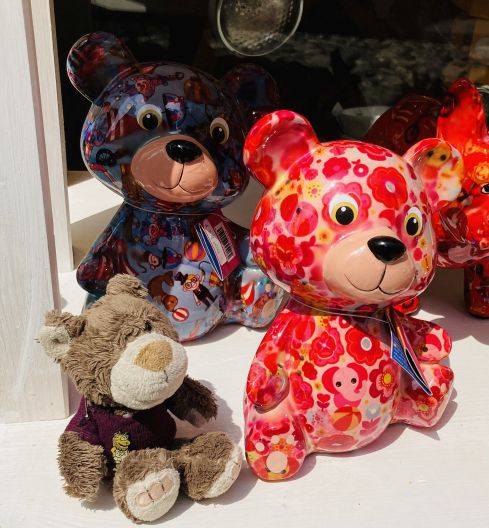
\includegraphics[width=4cm]{frame-bear-small}};
    
    \node[fill=white] at (0.7,0.6) (bearcolor){\phantom{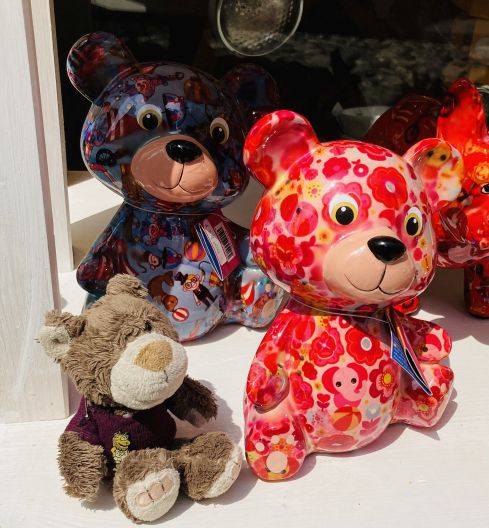
\includegraphics[width=4cm]{frame-bear-small}}};
   
    \begin{scope}[x=1cm,y=1cm,shift={(0.6\textwidth,0\textheight)}]
    % \path[red,draw](0,0)rectangle (5,5); 
    \choosecolor
     \path(bearcolor.south)--++(0,0.5) pic[scale=1.5,bear/body=bearcolor]{bear};
 
 	\draw[brown!80!black,line width=15pt] (bears.south east) rectangle (bears.north west);		
	\draw[brown!60!black,line width=10pt] (bears.south east) rectangle (bears.north west);	
	\draw[brown!80!black,line width=15pt] (bearcolor.south east) rectangle (bearcolor.north west);		
	\draw[brown!60!black,line width=10pt] (bearcolor.south east) rectangle (bearcolor.north west);	
 
     \pig[back,shift={(3,1)},rotate=
     %\fpeval{(5-\csname int_mod:nn\endcsname{\thepage}{10})}
     5*\fpeval{sin(\value{page}/50*2*pi)}
     ]
 
    \end{scope} 
    
    % credit for background image
    \node[white,text width=.7\paperwidth,font=\tiny,align=center] at ([yshift=0.35cm]current page.south) {Image source: private photo};  
    
  \end{tikzpicture}
  \pause[60]
\end{frame}	
	
\end{document}
